\documentclass{standalone}
\usepackage{tikz}
\usepackage{tabularx}
\usepackage{colortbl}
\usepackage{booktabs}

\begin{document}
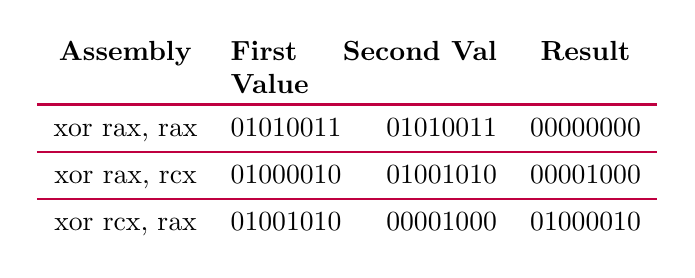
\begin{tikzpicture}

\node (tbl) {
\begin{tabularx}{.65\textwidth}{cXrcc}
\arrayrulecolor{purple}
\textbf{Assembly} & \textbf{First Value} & \textbf{Second Val} & \textbf{Result} \\
\toprule
xor rax, rax & 01010011 & 01010011 & 00000000 \\ 
\midrule
xor rax, rcx & 01000010 & 01001010 & 00001000 \\
\midrule
xor rcx, rax & 01001010 & 00001000 & 01000010 \\
\end{tabularx}
};

\end{tikzpicture}
\end{document}